\begin{figure}[htbp]\centering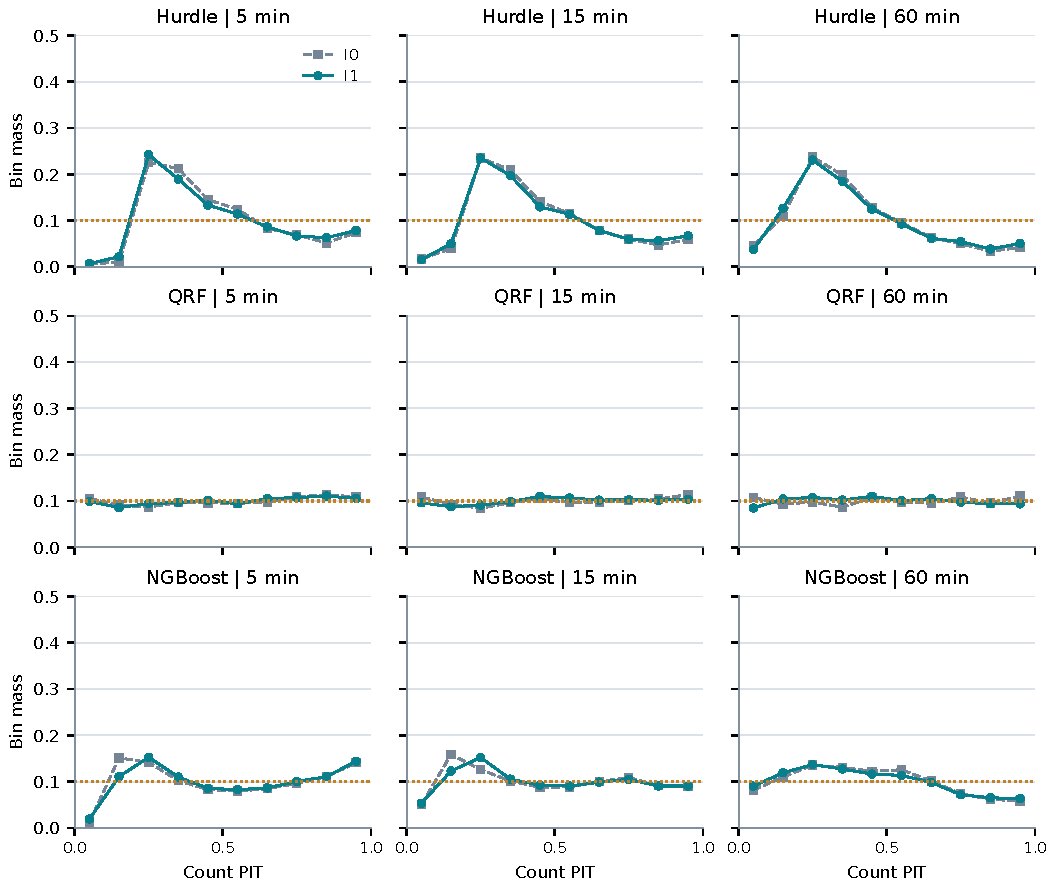
\includegraphics[width=\linewidth]{figures/pit_weibo_nonrandomized.pdf}\caption{Weibo: nonrandomized count PIT by family and prefix. The horizontal dotted line is 0.1. Seeds are averaged as prescribed; the panels are descriptive and do not add independent test cases.}\end{figure}
\clearpage\begin{figure}[htbp]\centering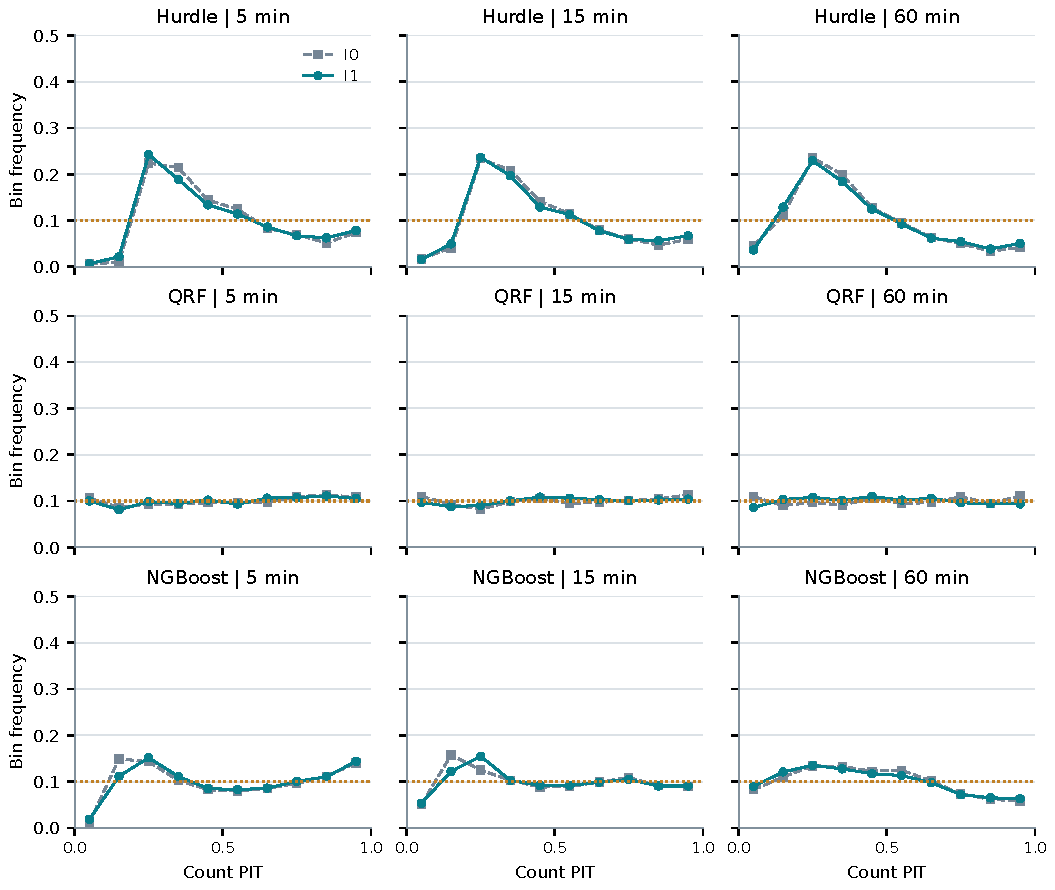
\includegraphics[width=\linewidth]{figures/pit_weibo_randomized.pdf}\caption{Weibo: randomized count PIT by family and prefix. The horizontal dotted line is 0.1. Seeds are averaged as prescribed; the panels are descriptive and do not add independent test cases.}\end{figure}
\clearpage\begin{figure}[htbp]\centering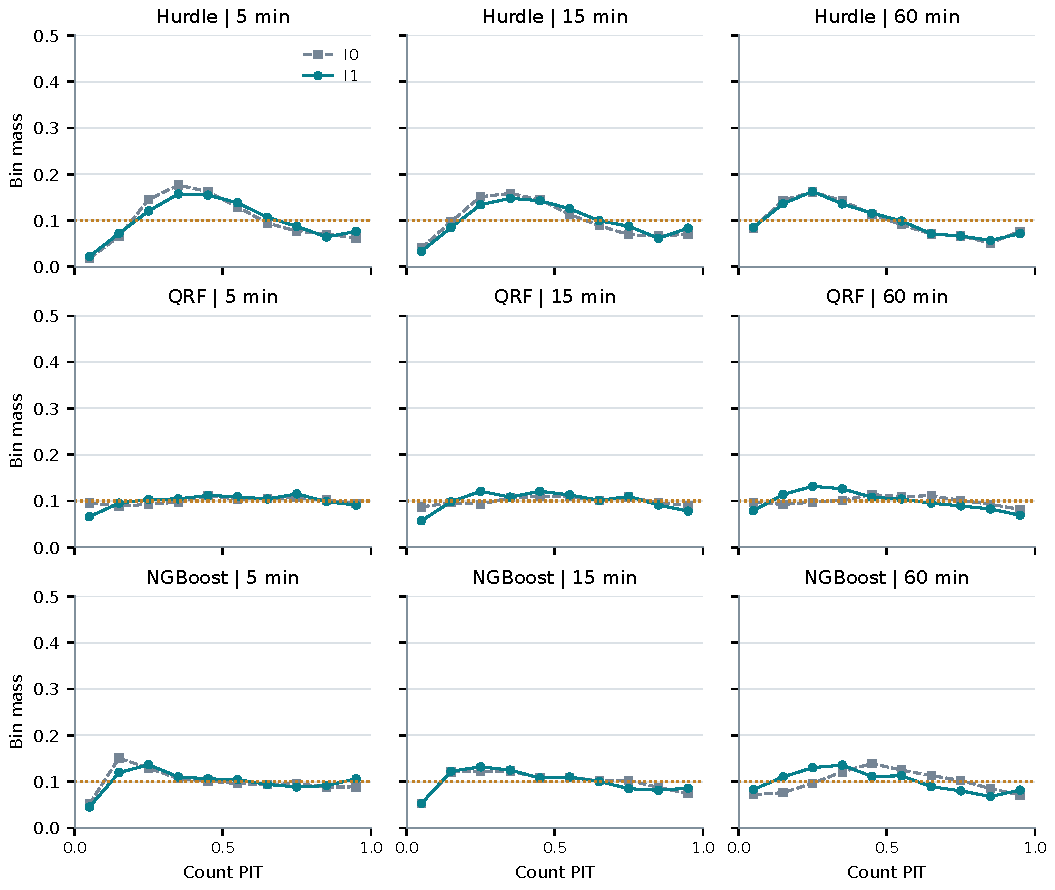
\includegraphics[width=\linewidth]{figures/pit_seismic_nonrandomized.pdf}\caption{SEISMIC: nonrandomized count PIT by family and prefix. The horizontal dotted line is 0.1. Seeds are averaged as prescribed; the panels are descriptive and do not add independent test cases.}\end{figure}
\clearpage\begin{figure}[htbp]\centering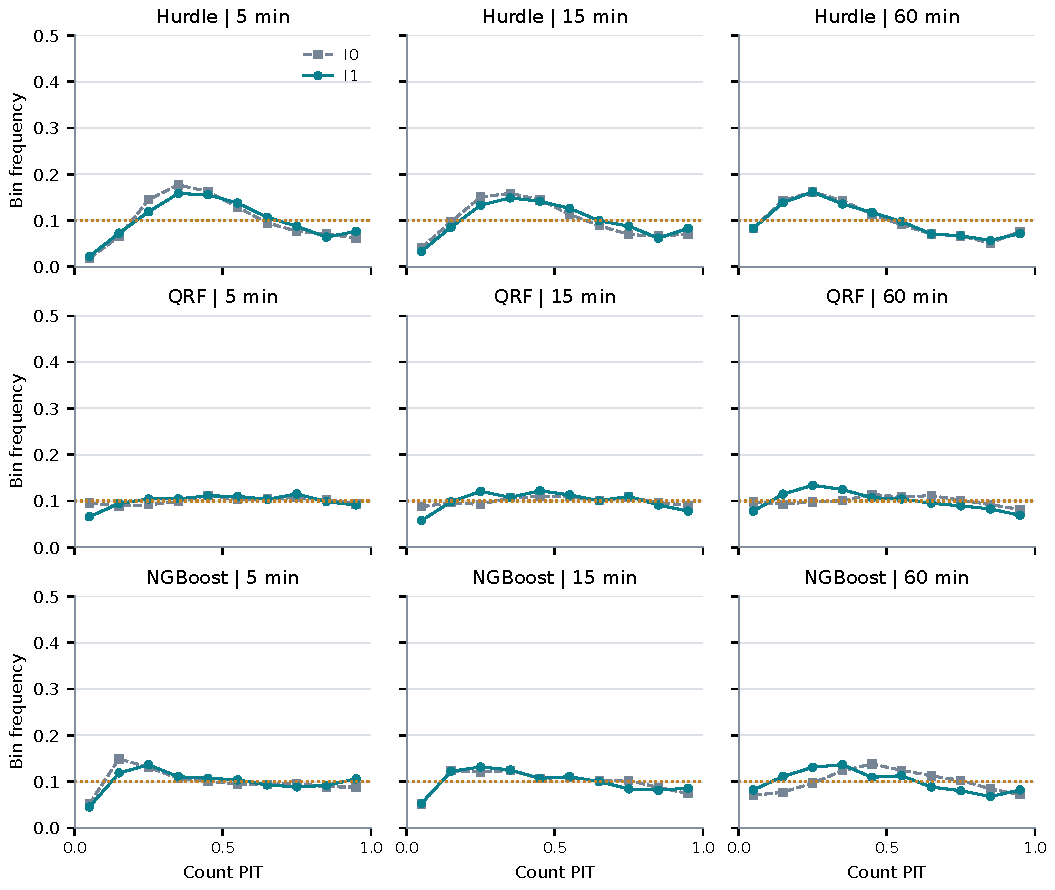
\includegraphics[width=\linewidth]{figures/pit_seismic_randomized.pdf}\caption{SEISMIC: randomized count PIT by family and prefix. The horizontal dotted line is 0.1. Seeds are averaged as prescribed; the panels are descriptive and do not add independent test cases.}\end{figure}
\clearpage\begin{figure}[htbp]\centering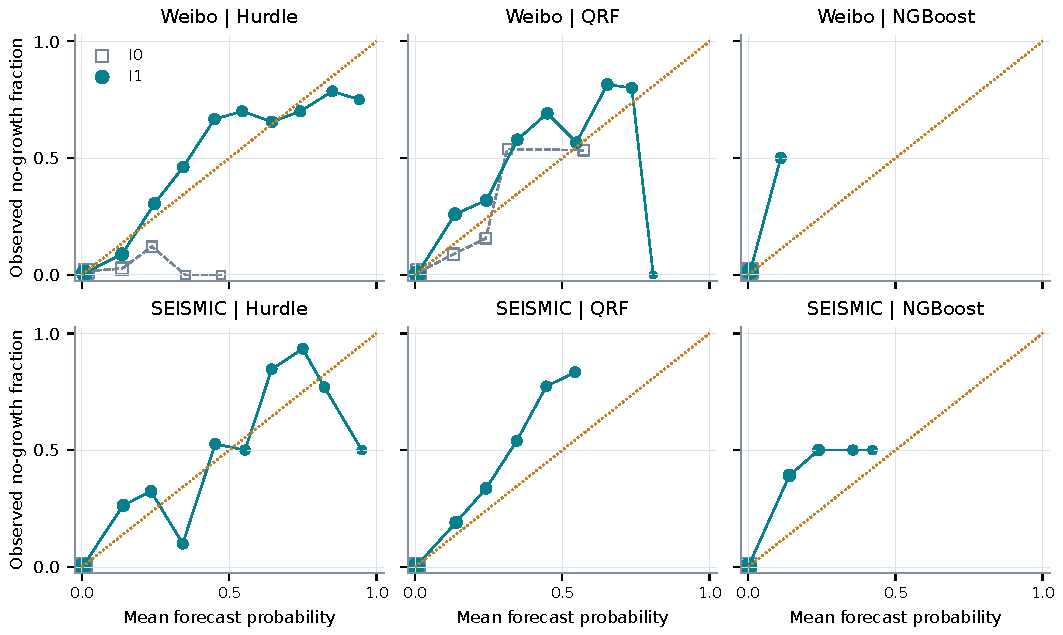
\includegraphics[width=\linewidth]{figures/no_growth_reliability.pdf}\caption{Aggregate no-growth reliability. Only occupied fixed bins are shown. Marker area increases with the logarithm of the saved bin count; counts reflect the prescribed averaging over seeds. Sparse high-probability bins remain descriptive. The diagonal is equality.}\end{figure}